\section{Methode}
Vestibulum viverra auctor elit et sodales. Vivamus vitae molestie ipsum. Mauris vel augue eu est scelerisque tempus vitae id justo. Etiam eu dui sed lorem placerat finibus vel quis tellus. Maecenas tristique dolor lectus, vitae egestas nisi vulputate et. Pellentesque tincidunt sapien nec libero fermentum rhoncus. Aliquam porta consequat sapien sit amet fermentum. Nunc pellentesque imperdiet tellus, ac condimentum eros elementum molestie.
%Met een witregel tussen de alinea 's zal de volgende regel inspringen
Curabitur cursus finibus lectus in dignissim. Sed pellentesque, nisi in blandit iaculis, eros purus interdum leo, quis dictum purus mi a est. Nullam in magna id lacus ultrices porttitor. Curabitur finibus ipsum nec dui semper bibendum. Suspendisse bibendum ante sed feugiat dignissim. \\

%Door \\ aan het einde van een alinea zal er een witregel tussen de alinea 's komen. Om dan te voorkomen dat de tekst ook nog inspringt gebruik je het commando no indent
\noindent Vivamus nec urna lacus. Praesent at fringilla elit. Phasellus fringilla dolor id metus sodales lobortis. Pellentesque tincidunt nec magna a rhoncus. Etiam auctor pulvinar rutrum. Morbi vel nulla nisl. Etiam convallis condimentum libero et rhoncus. Ut a hendrerit erat. Vivamus vel posuere massa. Fusce aliquam purus ut fermentum sollicitudin. Ut ut accumsan diam \footnote{Dit is een footnote}. %Zo maak je een footnote aan.

\subsection{Participanten}
Lorem ipsum dolor sit amet, consectetur adipiscing elit. Quisque gravida justo eu urna suscipit posuere. Nulla euismod purus sapien, vel fermentum orci pharetra pharetra. Aenean aliquam nulla vel tellus luctus, quis efficitur neque condimentum. Sed lacinia dictum ex, ac mollis arcu consectetur sit amet. Duis pharetra risus tincidunt nisi consequat condimentum. Praesent malesuada dapibus elit at suscipit.

%Op deze manier kunnen er twee afbeeldingen naast elkaar. 
\begin{figure}[H]
    \begin{minipage}[p]{0.48\textwidth}
        \centering
        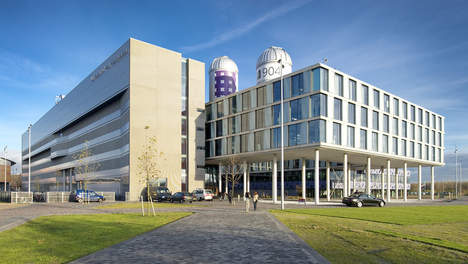
\includegraphics[width=0.95\textwidth]{SciencePark.jpg}
    \end{minipage}
    \begin{minipage}[p]{0.48\textwidth}
        \centering
        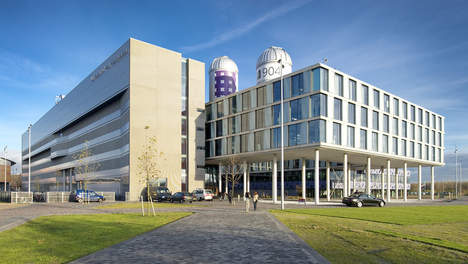
\includegraphics[width=0.95\textwidth]{SciencePark.jpg}
    \end{minipage}
    \caption{Science Park}
\end{figure}

%Zo gebruik je een losse afbeelding.
\begin{figure}[H]
    \centering
        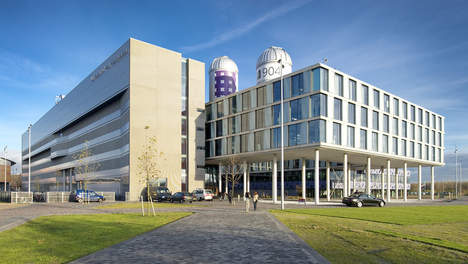
\includegraphics[width=0.7\textwidth]{SciencePark.jpg}
        \caption{Science Park}
        \centering
\end{figure}


\subsection{Procedure}
%Hierdoor wordt er een lijst aangemaakt, verdeeld over twee kolommen
\begin{itemize}
\begin{multicols}{2} %Hier geef je het aantal kolommen aan
    \item{item 1}
    \item{item 2}
    \item{item 3}
    \item{item 4}
    \item{item 5}
    \item{item 6}
\end{multicols}
\end{itemize}

\subsection{Analyse}
%Ook de tekst kan in twee kolommen gezet worden
\begin{multicols}{2}
Donec quis nisl fermentum, luctus ligula ac, interdum neque. Praesent a justo sit amet nisl aliquet consectetur nec et ipsum. Curabitur porttitor felis vitae turpis egestas, mattis congue mi pretium. Phasellus eu felis a metus accumsan sollicitudin sed non diam. Sed consectetur, ligula ut pellentesque laoreet, mauris nisi rutrum enim, a maximus metus massa eget felis. Donec ac ultricies arcu. Sed ultricies non sem ut molestie. Suspendisse lacinia dolor in egestas gravida. Donec ut porttitor massa, sit amet aliquet ex. Proin sit amet dui eget turpis elementum luctus sed a nibh.
\end{multicols}
